\section{Methodology and Implementation}
% What were the methods used?
% How was the problem designed?
% Driving concepts
% Equations
% Figures

A modular, agent-based is an ideal approach for solving complicated
physics-dependent supply chain problems involving material routing, facility
deployment, regional and institutional hierarchies.

\subsection{Framework Structure}
% (OO, cpp, xml, backends, inheritances, mixins, generic apis, etc.)

Agent-based modeling is inherently object oriented. 

The core of the simulator creates a set of key classes on which agent plugins 
are based. In addtion, a set of key tools are also provided, to enrich the API 
and provide a robust suite of behaviors for the developer.

<diagram of core, modules, toolkit, etc>

Agent plug-ins utilize the generic core API to interact with one another. 
Mainly they do this by trading resources. 

<diagram of black box facilities>

\subsection{Cluster-Ready Software}

Because this doesn't rely on PowerSim, GoldSim, Excel, or any other COTS 
Windows-based software, we can run singular instances of Cyclus 
on large linux machines that have lots more capability than hacked together 
Windows clusters. 

\subsection{Dynamically Loadable Libraries}
% (diagram)

A key innovation that has previously not been implemented in nuclear fuel cycle 
simulators in the literature is implementing this generic API and modular 
architecture into a suite of dynamically loadable ``plug-in'' libraries. 
This is implemented largely through a clean API and a modern build system.

Dynamically-loadable libraries are the primary mechanism for extending \Cyclus' capability. 
This approach provides encapsulation: the core of the code operates
completely independently from the individual libraries. Thus, any
customization or extension is implemented only in the loadable
library. 

This approach allows efficient, targeted contribution to the ecosystem of libraries.  The 
scientist-developer can therefore focus on generating a model within their 
sphere of expertise, while relying on the model contributions of others to fill 
in the other technologies.  This strategy also allows individual developers to
explore different levels of complexity within their archetypes, including
wrapping other simulation tools as loadable libraries within the \Cyclus
framework.

A secondary benefit is the ability for
contributors to choose different distribution and licensing strategies
for their contributions. By allowing models to have varied
availability, the security concerns of developers can be
assuaged (See Figure \ref{fig:modifiedopen}).

\begin{figure}[htbp!]
\begin{center}
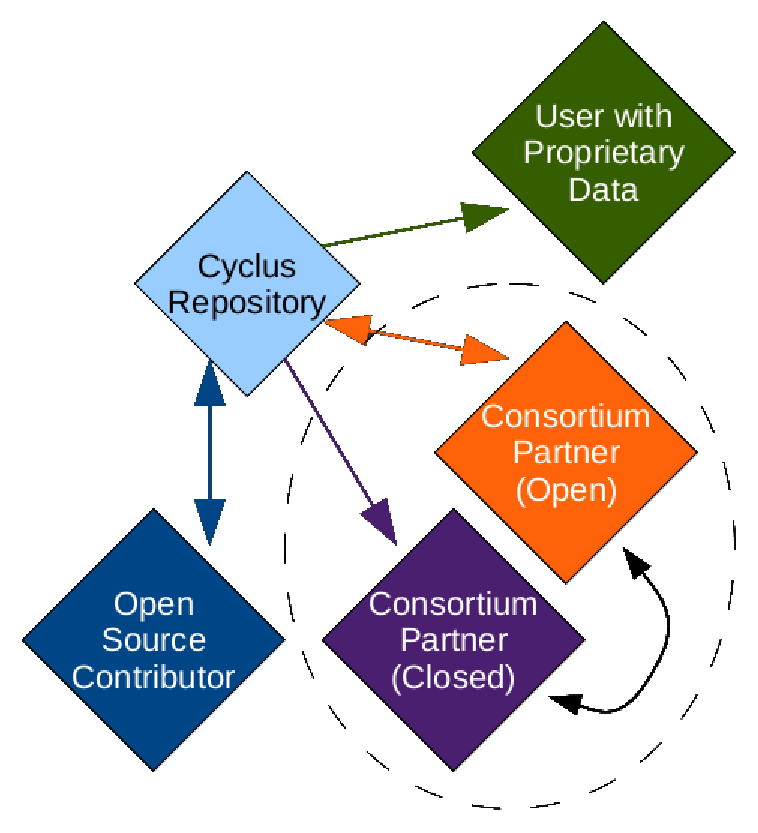
\includegraphics{./images/modifiedopen.eps}
\end{center}
\caption{The \Cyclus framework enables fully open, partially open, and fully
closed collaborations\cite{wilson_cyclus:_2012}.}
\label{fig:modifiedopen}
\end{figure}

In particular, since the clean plug-in architecture loads libraries without any
modifications to the \Cyclus kernel, closed-source archetypes can be used with
the simulator alongside open-source archetypes. This architecture therefore
allows closed-source libraries (e.g., those representing sensitive nuclear
processes and subject to export control) to be developed and licensed privately.

This last benefit of dynamically-loadable libraries addresses
another goal of \Cyclus: ubiquity amongst its potential user base. By
engineering \Cyclus to easily handle varying levels of complexity, a single
simulation engine can be used by both users interested in big-picture policy
questions as well as users focused on more detailed, technical
analyses.


\subsection{Agent Interchangability}
% interchangeability due to exchange behavior api

This approach enables ``apples-to-apples'' comparisons, something that has been 
sorely missing in previous simulators.

By making the facilities interchangeable, it combinatorically increases the 
number of scenarios that can be modeled. The user can choose to model just the 
front end or just the back end of a fuel cycle. 

This is implemented with an API that focuses on treating the agents as black 
boxes. 

\subsection{Regions, Institutions, and Facilities}

\Cyclus provides a novel representation of entities in the nuclear fuel cycle,
including facilities, institutions managing those facilities, and regions. While
some simulators (TODO cite DESAE) have provided a notion of static regional
effects, \Cyclus allows for both regions and institutions to be first-class
actors in simulated fuel cycles.

Cyclus has three core agent classes that be subclassed to create a simulation
archetype: Region, Institution, and Facility. At present, Regions, Institutions,
and Facilities (RIF) conceptually form a nested structure in a Cyclus simulation,
i.e., Facilities exist in (i.e., are managed by) Institutions and Institutions
exist in Regions.

Importantly, the RIF separation allows for preferential trading. For example,
Facilities in the same Institution can preferentially trade with each
other. Similarly, Regions can be given a location proxy, and the trade between
Facilities can be informed by their regional proximity.

\subsection{Discrete Object Tracking}
% Resources, Materials (note isotope tracking, decay behavior)

Discrete facility and material tracking is more realistic an dmore 

\subsection{Toolkit}
% library of tools
% contributions to the toolkit
% place for metrics

The toolkit is a place for developers and users to contribute common-use tools 
for calculating metrics, managing process physics, and handling data.

This was implemented by liberal use of namespaces and is populated with an
introductory suite of useful tools, including helper classes for managing
facility deployment, minimum cost facility deployment decision making, and for
enrichment-related calculations.

\subsection{Cycamore}
% base modules

Cycamore contains a number of useful facility models that are a mere base-set.
Additional modules are needed for interesting fuel cycle simulation. However,
simple, once-through fuel cycles can be generated with Cycamore and Cyclus alone.

<diagram of a possible Cycamore-only simulation>
